\documentclass[12pt]{report}
\usepackage[utf8]{inputenc}
\usepackage[russian]{babel}
%\usepackage[14pt]{extsizes}
\usepackage{listings}
\usepackage{graphicx}
\usepackage{amsmath,amsfonts,amssymb,amsthm,mathtools} 
\usepackage{pgfplots}
\usepackage{filecontents}
\usepackage{indentfirst}
\usepackage{eucal}
\usepackage{enumitem}
\frenchspacing

\usepackage{indentfirst} % Красная строка


\usetikzlibrary{datavisualization}
\usetikzlibrary{datavisualization.formats.functions}

\usepackage{amsmath}




% Для листинга кода:
\lstset{ %
language=python,                 % выбор языка для подсветки
basicstyle=\small\sffamily, % размер и начертание шрифта для подсветки кода
numbers=left,               % где поставить нумерацию строк (слева\справа)
numberstyle=\tiny,           % размер шрифта для номеров строк
stepnumber=1,                   % размер шага между двумя номерами строк
numbersep=5pt,                % как далеко отстоят номера строк от подсвечиваемого кода
showspaces=false,            % показывать или нет пробелы специальными отступами
showstringspaces=false,      % показывать или нет пробелы в строках
showtabs=false,             % показывать или нет табуляцию в строках
frame=single,              % рисовать рамку вокруг кода
tabsize=2,                 % размер табуляции по умолчанию равен 2 пробелам
captionpos=t,              % позиция заголовка вверху [t] или внизу [b] 
breaklines=true,           % автоматически переносить строки (да\нет)
breakatwhitespace=false, % переносить строки только если есть пробел
escapeinside={\#*}{*)}   % если нужно добавить комментарии в коде
}

\usepackage[left=2cm,right=2cm, top=2cm,bottom=2cm,bindingoffset=0cm]{geometry}
% Для измененных титулов глав:
\usepackage{titlesec, blindtext, color} % подключаем нужные пакеты
\definecolor{gray75}{gray}{0.75} % определяем цвет
\newcommand{\hsp}{\hspace{20pt}} % длина линии в 20pt
% titleformat определяет стиль
\titleformat{\chapter}[hang]{\Huge\bfseries}{\thechapter\hsp\textcolor{gray75}{|}\hsp}{0pt}{\Huge\bfseries}


% plot
\usepackage{pgfplots}
\usepackage{filecontents}
\usetikzlibrary{datavisualization}
\usetikzlibrary{datavisualization.formats.functions}

\begin{document}
\thispagestyle{empty}
\begin{titlepage}
	\noindent \begin{minipage}{0.15\textwidth}
	
\includegraphics[width=\linewidth]{b_logo}
	\end{minipage}
	\noindent\begin{minipage}{0.9\textwidth}\centering
		\textbf{Министерство науки и высшего образования Российской Федерации}\\
		\textbf{Федеральное государственное бюджетное образовательное учреждение высшего образования}\\
		\textbf{~~~«Московский государственный технический университет имени Н.Э.~Баумана}\\
		\textbf{(национальный исследовательский университет)»}\\
		\textbf{(МГТУ им. Н.Э.~Баумана)}
	\end{minipage}
	
	\noindent\rule{18cm}{3pt}
	\newline\newline
	\noindent ФАКУЛЬТЕТ $\underline{\text{«Информатика и системы управления»}}$ \newline\newline
	\noindent КАФЕДРА $\underline{\text{«Программное обеспечение ЭВМ и информационные технологии»}}$\newline\newline\newline\newline\newline
	
	
	\begin{center}
		\noindent\begin{minipage}{1.3\textwidth}\centering
			\Large\textbf{  Отчет по лабораторной работе №2}\newline
			\textbf{по дисциплине "Анализ алгоритмов"}\newline\newline
		\end{minipage}
	\end{center}
	
	\noindent\textbf{Тема} $\underline{\text{Алгоритмы умножения матриц}}$\newline\newline
	\noindent\textbf{Студент} $\underline{\text{Андрич К. }}$\newline\newline
	\noindent\textbf{Группа} $\underline{\text{ИУ7И-56Б}}$\newline\newline
	\noindent\textbf{Оценка (баллы)} $\underline{\text{~~~~~~~~~~~~~~~~~~~~~~~~~~~}}$\newline\newline
	\noindent\textbf{Преподаватели} $\underline{\text{Волкова Л.Л.}}$\newline\newline\newline
	
	\begin{center}
		\vfill
		Москва~---~\the\year
		~г.
	\end{center}
\end{titlepage}


\tableofcontents

\newpage
\chapter*{Введение}
\addcontentsline{toc}{chapter}{Введение}
Термин «матрица» применяется во множестве разных областей: от программирования до кинематографии.
\newline

Матрица в математике – это таблица чисел, состоящая из определенного количества строк (m) и столбцов (n).
\newline

Мы встречаемся с матрицами каждый день, так как любая числовая информация, занесенная в таблицу, уже в какой-то степени считается матрицей.
\newline

Примером могут служить:

\begin{itemize}
	\item список телефонных номеров;
	\item различные статистические данные;
	\item табель успеваемости ученика и многое другое.
\end{itemize}

Целью работы работы является изучение и реализация алгоритмов умножения матриц, вычисление трудоёмкости этих алгоритмов. В данной лабораторной работе рассматривается стандартный алгоритм умножения матриц, алгоритм Винограда и модифицированный алгоритм Винограда.
\newline

Для достижения цели ставятся следующие задачи.
\begin{itemize}
	\item Изучить классический алгоритм умножения матриц, алгоритм Винограда и модифицированный алгоритм Винограда.
	\item Реализовать классический алгоритм умножения матриц, алгоритм Винограда и модифицированный алгоритм Винограда.
	\item Дать оценку трудоёмкости алгоритмов.
	\item Замерить время работы алгоритмов.
	\item Описать и обосновать полученные результаты в отчете о выполненной лабораторной
	работе, выполненном как расчётно-пояснительная записка к работе. 
\end{itemize}

\chapter{Аналитическая часть}

\textbf{Матрица} – математический объект, эквивалентный двумерному массиву. Числа располагаются в матрице по строкам и столбцам. Две матрицы одинакового размера можно поэлементно сложить или вычесть друг из друга.
\newline

Если число столбцов в первой матрице совпадает с числом строк во второй, то эти две матрицы можно перемножить. У произведения будет столько же строк, сколько в первой матрице, и столько же столбцов, сколько во второй. При умножении матрицы размером 3х4 на матрицу размером 4x7 мы получаем матрицу размером 3x7. Умножение матриц некоммутативно: оба произведения АВ и ВА двух квадратных матриц одинакового размера можно вычислить, однако результаты, вообще говоря, будут отличаться друг от друга.

\section{Классический алгоритм умножения матриц}

Пусть даны две прямоугольные матрицы А (\ref{bmtr:matrixa}) и В (\ref{bmtr:matrixb}) размерности m на n и n на p соответсвенно: 
\begin{equation}
	\label{bmtr:matrixa}
	\begin{bmatrix}
		a_{1,1} & ... & a_{1,n} \\
		... & ... & ... \\
		a_{m,1} & ... & a_{m,n} \\
	\end{bmatrix} \\
\end{equation}

\begin{equation}
	\label{bmtr:matrixb}
	\begin{bmatrix}
		b_{1,1} & ... & b_{1,p} \\
		... & ... & ... \\
		b_{n,1} & ... & b_{n,p} \\
	\end{bmatrix} \\
\end{equation}

В результате получим матрицу C (\ref{bmtr:matrixc}) размерности m на p:

\begin{equation}
	\label{bmtr:matrixc}
	\begin{bmatrix}
		c_{1,1} & ... & c_{1,p} \\
		... & ... & ... \\
		c_{m,1} & ... & c_{m,p} \\
	\end{bmatrix} \\
\end{equation}

Формула (\ref{bmtr:cij}) - формула рассчёта элемента, находящегося на i-ой строке j-ого столбца матрицы C.

\begin{equation}
	\label{bmtr:cij}
	c_{i,j} = \sum\limits_{r=1}^n a_{i,r}\cdot b_{r,j}
\end{equation}

\section{Алгоритм Винограда}

Если посмотреть на результат умножения двух матриц, то видно, что каждый элемент в нем представляет собой скалярное произведение соответствующих строки и столбца исходных матриц. Можно заметить также, что такое умножение допускает предварительную обработку, позволяющую часть работы выполнить заранее.

Рассмотрим два вектора $V = (v1, v2, v3, v4)$ и $W = (w1, w2, w3, w4)$. Их скалярное произведение (\ref{eq:dot}) равно: 

\begin{equation}
	\label{eq:dot}
	V \cdot W=v_1 \cdot w_1 + v_2 \cdot w_2 + v_3 \cdot w_3 + v_4 \cdot w_4\\
\end{equation}
\newline

Это равенство можно переписать в виде (\ref{eq:dot1}):

\begin{equation}
	\label{eq:dot1}
	V \cdot W=(v_1 + w_2) \cdot (v_2 + w_1) + (v_3 + w_4) \cdot (v_4 + w_3) - v_1 \cdot v_2 - 
	v_3 \cdot v_4 - w_1 \cdot w_2 - w_3 \cdot w_4
\end{equation}

Менее очевидно, что выражение в правой части последнего равенства допускает предварительную обработку: его части можно вычислить заранее и запомнить для каждой строки первой матрицы и для каждого столбца второй. 
Это означает, что над предварительно обработанными элементами нам придется выполнять лишь первые два умножения и последующие пять сложений, а также дополнительно два сложения.

\section{Оптимизированный алгоритм Винограда}
Оптимизированный алгоритм Винограда представляет собой обычный алгоритм Винограда, за исключением следующих оптимизаций:

\begin{itemize}
	\item вычисление происходит заранее;
	\item используется битовый сдвиг, вместо деления на 2;
	\item последний цикл для нечётных элементов включён в основной цикл, используя дополнительные операции в случае нечётности N.
\end{itemize}

\section{Вычисление трудоёмкости алгоритма}
Введем модель трудоемкости для оценки алгоритмов.
\begin{enumerate}
	\item  Базовые операции стоимостью 1: +, -, *, /, =, ==, <=, >=, !=, +=, [], получение полей класса.
	\item Оценка трудоемкости цикла: f\_цикла = f\_инициализации + f\_сравнения + N * (f\_инкремента + f\_сравнения + f\_тела).
	\item Стоимость условного перехода возьмем за 0, стоимость вычисления условия остаётся. В условном операторе может возникнуть лучший и худший случаи по трудоёмкости в зависимости от выполнения условия и в зависимости от входных данных алгоритма.
\end{enumerate}

\section{Вывод}
	В данном разделе были рассмотрены алгоритмы классического умножения матриц и алгоритм Винограда, основная разница которого — наличие предварительной обработки, а также уменьшение количества операций умножения. 
	
\clearpage

\chapter{Конструкторская часть}

\section{Схемы алгоритмов}

На рисунке \ref{fig:base} представлена схема классического умножения матриц.

\begin{figure}[h]
	\centering
	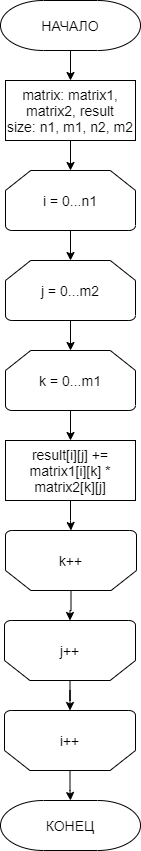
\includegraphics[width=0.145\linewidth]{base.jpg}
	\caption{Схема классического алгоритма умножения матриц}
	\label{fig:base}
\end{figure}

На рисунках \ref{fig:vin1}, \ref{fig:vin2}, \ref{fig:vin3}, \ref{fig:vin4} представлена схема алгоритма умножения матриц Винограда.

\begin{figure}[h]
	\centering
	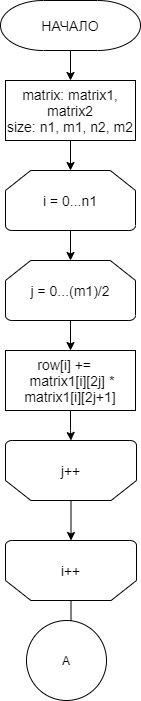
\includegraphics[width=0.202\linewidth]{vin1.jpg}
	\caption{Схема алгоритма Винограда (часть 1)}
	\label{fig:vin1}
\end{figure}

\newpage

\begin{figure}[h]
	\centering
	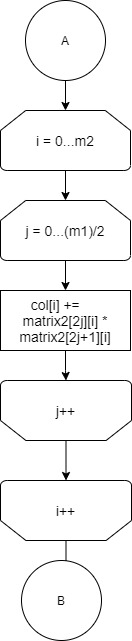
\includegraphics[width=0.207\linewidth]{vin2.jpg}
	\caption{Схема алгоритма Винограда (часть 2)}
	\label{fig:vin2}
\end{figure}

\newpage

\begin{figure}[h]
	\centering
	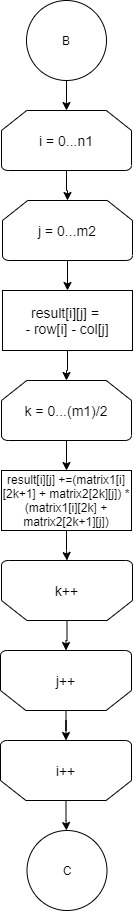
\includegraphics[width=0.146\linewidth]{vin3.jpg}
	\caption{Схема алгоритма Винограда (часть 3)}
	\label{fig:vin3}
\end{figure}

\newpage

\begin{figure}[h]
	\centering
	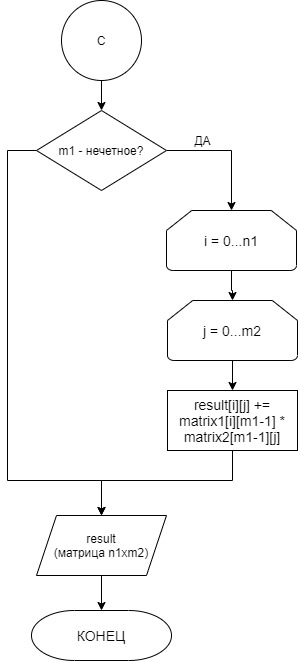
\includegraphics[width=0.4\linewidth]{vin4.jpg}
	\caption{Схема алгоритма Винограда (часть 4)}
	\label{fig:vin4}
\end{figure}

\newpage

На рисунках \ref{fig:vinOpt1}, \ref{fig:vinOpt2}, \ref{fig:vinOpt3}, \ref{fig:vinOpt4} представлена схема оптимизированного алгоритма умножения матриц Винограда.

\begin{figure}[h]
	\centering
	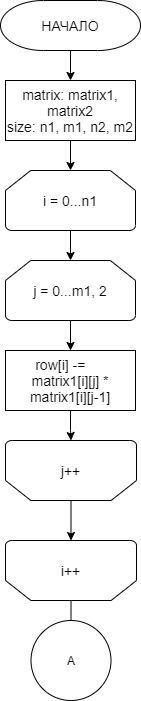
\includegraphics[width=0.202\linewidth]{vinopt1.jpg}
	\caption{Схема оптимизированного алгоритма Винограда(часть 1)}
	\label{fig:vinOpt1}
\end{figure}

\newpage

\begin{figure}[h]
	\centering
	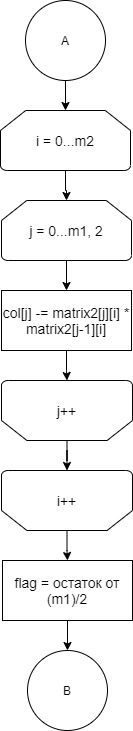
\includegraphics[width=0.18\linewidth]{vinopt2.jpg}
	\caption{Схема оптимизированного алгоритма Винограда(часть 2)}
	\label{fig:vinOpt2}
\end{figure}

\newpage

\begin{figure}[h]
	\centering
	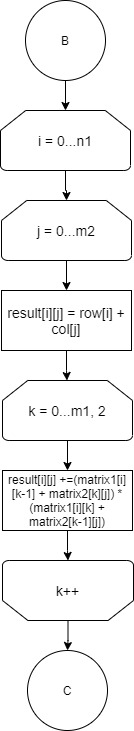
\includegraphics[width=0.18\linewidth]{vinopt3.jpg}
	\caption{Схема оптимизированного алгоритма Винограда(часть 3)}
	\label{fig:vinOpt3}
\end{figure}

\newpage 

\begin{figure}[h]
	\centering
	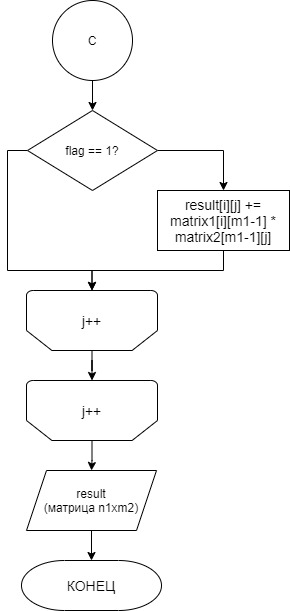
\includegraphics[width=0.4\linewidth]{vinopt4.jpg}
	\caption{Схема оптимизированного алгоритма Винограда(часть 4)}
	\label{fig:vinOpt4}
\end{figure}

\newpage

\section{Оценка трудоемкости алгоритмов умножения матриц}
\hfill
\begin{enumerate}
	\item Стандартный алгоритм
	$$f=2+M(2+2+Q(2+2+N(2+8+1+1+1)))=13 \cdot$$
	
	$$\cdot MNQ+4MQ+4M+2 \approx 13 \cdot MNQ$$ 
	
	\item Алгоритм Винограда
	
	Трудоемкость алгоритма Винограда:\\
	
	Первый цикл: $\frac{15}{2} \cdot N  Q + 5 \cdot M + 2$ \\
	
	Второй цикл: $\frac{15}{2} \cdot M  N + 5 \cdot M + 2$\\
	
	Третий цикл: $13 \cdot M  N Q + 12 \cdot M Q + 4 \cdot M + 2$\\
	
	Условный переход: $\begin{bmatrix}
		2    &&, \text{лучший случай (при четном N)}\\
		15 \cdot QM + 4 \cdot M + 4 &&, \text{худший случай}\\
	\end{bmatrix} $ \\
	
	Итого: $f = \frac{15}{2} \cdot M  N + \frac{15}{2} \cdot Q  N + 9 \cdot M + 8 +  5 \cdot Q + 13 \cdot M  N Q + 12 \cdot M Q +
	\begin{bmatrix}
		2    &&, \text{в лучшем случае}\\
		15 \cdot QM + 4 \cdot M + 4 &&, \text{в худшем случае}\\
	\end{bmatrix} $ \\
	
	$$f \approx 13 \cdot MNQ $$
	
	\item Оптимизированный алгоритм Винограда
	
	Введем оптимизации: 
	\begin{enumerate}
		\item замена оперции = на += или -=
		\item избавление от деления в условиях цикла (j < N, j += 2)
		\item Заносим проверку на нечетность кол-ва строк внутрь основных циклов
		\item Расчет условия для последнего цикла один раз, а далее использование флага
	\end{enumerate}
	
	Первый цикл: $4 \cdot N  Q + 4 \cdot M + 2$ \\
	
	Второй цикл: $4 \cdot M  N + 4 \cdot M + 2$\\
	
	Третий цикл: $9 \cdot M  N Q + 10 \cdot M Q + 4 \cdot M + 2$\\
	
	Условный переход: $\begin{bmatrix}
		2   &&, \text{лучший случай (при четном N)}\\
		10 \cdot QM &&, \text{худший случай}\\
	\end{bmatrix} $ \\
	
	Трудоемкость оптимизированного алгоритма Винограда:\\
	
	Итого: $$f = 4 \cdot N  Q + 4 \cdot M + 2 + 4 \cdot M  N + 4 \cdot M + 2 + 9 \cdot M  N Q + 10 \cdot M Q + 4 \cdot M + 2 + $$
	
	$$ + \begin{bmatrix}
		2   &&, \text{л.c}\\
		10 \cdot QM &&, \text{х.c}\\
	\end{bmatrix} \approx 9 \cdot MNQ$$
	
	
\end{enumerate}

\section{Вывод}
	На основе теоретических данных, полученные в аналитическом разделе были построены схемы иследуеммых  алгоритмов.

\chapter{Технологическая часть}

\section{Выбор ЯП}
В данной лабораторной работе использовался язык программирования - python. Данный выбор обусловлен тем, что этот язык наиболее удобен для работы со строками, а также тем, что в нём присутсвует функция для измерения процессорного времени.
В качестве среды разработки я использовала Visual Studio Code, так как считаю его достаточно удобным.

\section{Требование к ПО}
\textbf{Требования к вводу:}
\begin{enumerate}
	\item На вход подаются две пустые матрицы - корректный ввод, программа не должна аварийно завершаться;
	\item ПО должно выводить полученную матрицу;
	\item ПО должно выводить потраченное время;
\end{enumerate}

\section{Реализация алгоритмов}

В листингах 3.1 - 3.3 приведена реализация алгоритмов умножения матриц.

\begin{lstlisting}[label=some-code,caption=Функция классического умножения матриц,language=Python]
def standart_multiplication(mtx1, mtx2):
	if len(mtx2) != len(mtx1[0]):
		print("Size error!")
		return -1
	else:
		n = len(mtx1)
		q = len(mtx2[0])
		m = len(mtx1[0])
		mtx3 = [[0] * q for i in range(n)]
	
		for i in range(0, n):
			for j in range(0, q):
				for k in range(0, m):
					mtx3[i][j] = mtx3[i][j] + mtx1[i][k] * mtx2[k][j]
	return mtx3
\end{lstlisting}

\begin{lstlisting}[label=some-code,caption=Функция умножения матриц с помощью аглоритма Винограда,language=Python]
def vinograd_multiplication(mtx1, mtx2):
	if len(mtx2) != len(mtx1[0]):
		print("Size error!")
		return -1
	else:
		m = len(mtx1)
		n = len(mtx1[0])
		q = len(mtx2[0])
		mtx3 = [[0] * q for i in range(m)]
		
		row = [0] * m
		for i in range(0, m):
			for j in range(0, n // 2, 1):
				row[i] = row[i] + mtx1[i][2 * j] * mtx1[i][2 * j + 1]
		
		col = [0] * q
		for j in range(0, q):
			for i in range(0, n // 2, 1):
				col[j] = col[j] + mtx2[2 * i][j] * mtx2[2 * i + 1][j]
		
		for i in range(0, m):
			for j in range(0, q):
				mtx3[i][j] = -row[i] - col[j]
				for k in range(0, n // 2, 1):
					mtx3[i][j] = mtx3[i][j] + (mtx1[i][2 * k + 1] + mtx2[2 * k][j]) * (mtx1[i][2 * k] + mtx2[2 * k + 1][j])
		
		if n % 2 == 1:
			for i in range(0, m):
				for j in range(0, q):
					mtx3[i][j] = mtx3[i][j] + mtx1[i][n - 1] * mtx2[n - 1][j]
		
	return mtx3
\end{lstlisting}

\newpage

\begin{lstlisting}[label=some-code,caption=Функция умножения матриц с помощью оптимизированного аглоритма Винограда,language=Python]
def vinograd_opt_multiplication(mtx1, mtx2):
	if len(mtx2) != len(mtx1[0]):
		print("Size error!")
		return -1
	else:
		m = len(mtx1)
		n = len(mtx1[0])
		q = len(mtx2[0])
		mtx3 = [[0] * q for i in range(m)]
		
		row = [0] * m
		for i in range(0, m):
			for j in range(1, n, 2):
				row[i] -= mtx1[i][j] * mtx1[i][j - 1]
		
		col = [0] * q
			for j in range(0, q):
				for i in range(1, n, 2):
					col[j] -= mtx2[i][j] * mtx2[i - 1][j]
		
		flag = n % 2
		for i in range(0, m):
			for j in range(0, q):
				mtx3[i][j] = row[i] + col[j]
				for k in range(1, n, 2):
					mtx3[i][j] += (mtx1[i][k - 1] + mtx2[k][j]) * (mtx1[i][k] + mtx2[k - 1][j])
				if (flag):
					mtx3[i][j] += mtx1[i][n - 1] * mtx2[n - 1][j]
	return mtx3
\end{lstlisting}

\section{Тестовые данные}

В таблице 3.1 приведены тестовые данные, на которых было протестированно разработанное ПО. Как видно из этой таблицы, все тесты были успешно пройдены, что означает, что программа работает правильно.

\begin{table}[h]
	\label{tabular:functional_test}
	\begin{center}
		\begin{tabular}{ | c | c | c | c |}
			\hline
			\textbf{Первая матрица} & \textbf{Вторая матрица} & \textbf{Ожидаемый результат} & \textbf{Полученный результат}\\ \hline
			$\begin{bmatrix} 
				1&2&3 \\
				4&5&6 \\ 
				7&8&9 \\ 
			\end{bmatrix}$ & 
			$\begin{bmatrix} 
				1&2&3 \\
				4&5&6 \\ 
				7&8&9 \\ 
			\end{bmatrix}$ &
			$\begin{bmatrix} 
				30&36&42 \\
				66&81&96 \\ 
				102&126&150 \\ 
			\end{bmatrix}$ &
			$\begin{bmatrix} 
				30&36&42 \\
				66&81&96 \\ 
				102&126&150 \\ 
			\end{bmatrix} $\\ 
			\hline
			
			
			$\begin{bmatrix} 
				1&2&3 \\
				4&5&6 \\ 
				7&8&9 \\ 
			\end{bmatrix}$ & 
			$\begin{bmatrix} 
				1&1&1 \\
				1&1&1 \\ 
			\end{bmatrix}$ &
			$\begin{matrix} 
				\text{Матрицы не могут} \\
				\text{быть перемножены} \\ 
			\end{matrix} $ &
			$\begin{matrix} 
				\text{Size error!} \\
			\end{matrix} $ \\
			\hline
			
			$\begin{bmatrix} 
				1&2 \\
				4&5 \\ 
				7&8 \\ 
			\end{bmatrix}$ & 
			$\begin{bmatrix} 
				1&2&3 \\
				4&5&6 \\ 
			\end{bmatrix}$ &
			$\begin{bmatrix} 
				9&12&15 \\
				24&33&42 \\ 
				39&54&69 \\ 
			\end{bmatrix} $ &
			$\begin{bmatrix} 
				9&12&15 \\
				24&33&42 \\ 
				39&54&69 \\ 
			\end{bmatrix} $ \\
			\hline
		\end{tabular}
		
	\end{center}
\end{table} 

\newpage

\section{Вывод}
В данном разделе были разработаны исходные коды трех алгоритмов: классическое умножение матриц, алгоритм Винограда, оптимизирвоанный алгоритм Винограда. 

\chapter{Исследовательская часть}

\section{Пример работы}

Демонстрация работы программы приведена на рисунке 4.1.

\begin{figure}[h]
	\begin{center}
	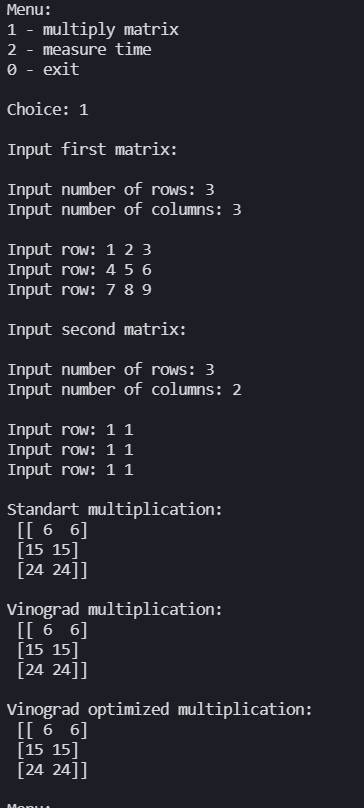
\includegraphics[scale=0.9]{example.png}
	 \caption{Работа алгоритмов умножения матриц.}
	\end{center}
\end{figure}

\section{Время выполнения алгоритмов}
Время выполнения алгоритмов замерялось с помощью функции process\_time модуля time в Python  \cite{process}. Данная функция возвращает значение в долях секунды суммы системного и пользовательского процессорного времени текущего процесса. \newline

В таблице 4.1. представлены замеры времени работы для каждого из алгоритмов.

\begin{table} [h!]
	\caption{Таблица времени выполнения алгоритмов}
	\begin{center}
		\begin{tabular}{|c c c c|} 
		 	\hline
			Длина строк & Standard & Vinograd & VinogradOpt \\  
		 	\hline
		 	100 & 0.515625 & 0.593750 & 0.406250 \\
		 	\hline
		 	200 & 4.000000 & 4.078125 & 3.296875 \\
		 	\hline
			300 & 13.625000 & 14.609375 & 11.093750 \\
			\hline
		\end{tabular}
	\end{center}
\end{table}

\begin{figure}[h!]
	\begin{center}
		\begin{tikzpicture}
			\begin{axis}[
				legend pos = north west,
				xlabel=длина строки,
				ylabel=секунды,
				minor tick num = 1,
				grid = both,
				major grid style = {lightgray},
				minor grid style = {lightgray!25},
				xtick distance = 50,
				width = 0.9\textwidth,
				height = 0.5\textwidth]
				
				\addplot[
				blue,
				semithick,
				mark = x,
				mark size = 3pt,
				thick,
				] file {Stand.txt};
				
				\addplot[
				red,
				semithick,
				mark = *,
				] file {Vin.txt};
				
				\legend{
					Классическое умножение,
					Алгоритм Винограда
				}
			\end{axis}
		\end{tikzpicture}
	\end{center}
	\caption{Сравнение классического умножения и умножения с помощю алгортима Винограда}
\end{figure}

\begin{figure}[h!]
	\begin{center}
		\begin{tikzpicture}
			\begin{axis}[
				legend pos = north west,
				xlabel=длина строки,
				ylabel=секунды,
				minor tick num = 1,
				grid = both,
				major grid style = {lightgray},
				minor grid style = {lightgray!25},
				xtick distance = 50,
				width = 0.9\textwidth,
				height = 0.5\textwidth]
				
				\addplot[
				blue,
				semithick,
				mark = x,
				mark size = 3pt,
				thick,
				] file {Vin.txt};
				
				\addplot[
				red,
				semithick,
				mark = *,
				] file {VinOpt.txt};
				
				\legend{
					Алгоритм Винограда,
					Оптимиризованный алгоритм Винограда
				}
			\end{axis}
		\end{tikzpicture}
	\end{center}
	\caption{Сравнение умножения с помощю алгортима Винограда и умножения с помощю оптимиризованного алгортима Винограда}
\end{figure}

\newpage


\section{Вывод}

В результате проведенного эксперимента был получен следующий вывод: оптимизированный алгоритм Винограда работает быстрее классического метода и зачительно быстрее обычного алгоритма Винограда.


\chapter*{Заключение}
\addcontentsline{toc}{chapter}{Заключение}

В ходе проделанной работы были изучены и реализованы классический алгоритм умножения матриц, алгоритм Винограда и модифицированный алгоритм Винограда. 

Экспериментально было подтверждено различие по временной эффективности алгоритмов умножения матриц на материале замеров процессорного времени выполнения реализации на варьирующихся размерах матриц. Так, самым быстрым является оптимизированный алгоритм Винограда,. Алгоритмы Винограда и классического умножения сопоставимы.

На основании сравнения данных алгоритмов был сделан вывод, что классический алгоритм является более эффективным, чем алгоритм Винограда, однако после ряда оптимизаций, алгоритм Винограда становится значительно быстрее классического. 

\addcontentsline{toc}{chapter}{Список литератури}

\bibliographystyle{utf8gost705u}  % стилевой файл для оформления по ГОСТу

\bibliography{51-biblio}          % имя библиографической базы (bib-файла)

\begin{thebibliography}{9}
	\addcontentsline{toc}{section}{Литература}
	\bibitem{matr}  Умножение матриц.[Электронный ресурс].Режим доступа: https://life-prog.ru/2\_90314\_umnozhenie-matrits.html (дата обращения: 25.09.2020)
	
	\bibitem{vinogr}  Умножение матриц по Винограду [электронный ресурс]. Режим доступа:
	
	http://algolib.narod.ru/Math/Matrix.html
	(дата обращения: 25.09.2020).
	
	\bibitem{python} Python documentation [Электронный ресурс]. Режим доступа:
	
	https://www.python.org/doc/
	(дата обращения: 26.09.2020).
	
\end{thebibliography}

\end{document}
